\section{Results}

\subsection{General Results}

After training the models, we evaluated their accuracies on the remaining trading, i.e., test data ranging from 01.11.2019 to 31.12.2019.
Before applying the models on the test data, we excluded bins for which no volume was traded, as we already did for the training data.
The accuracy for each model specification are illustrated below in figure \ref{fig:all_missing_bins_total}.

\begin{figure}[H]
    \captionsetup{format=plain}
    \makebox[\textwidth]{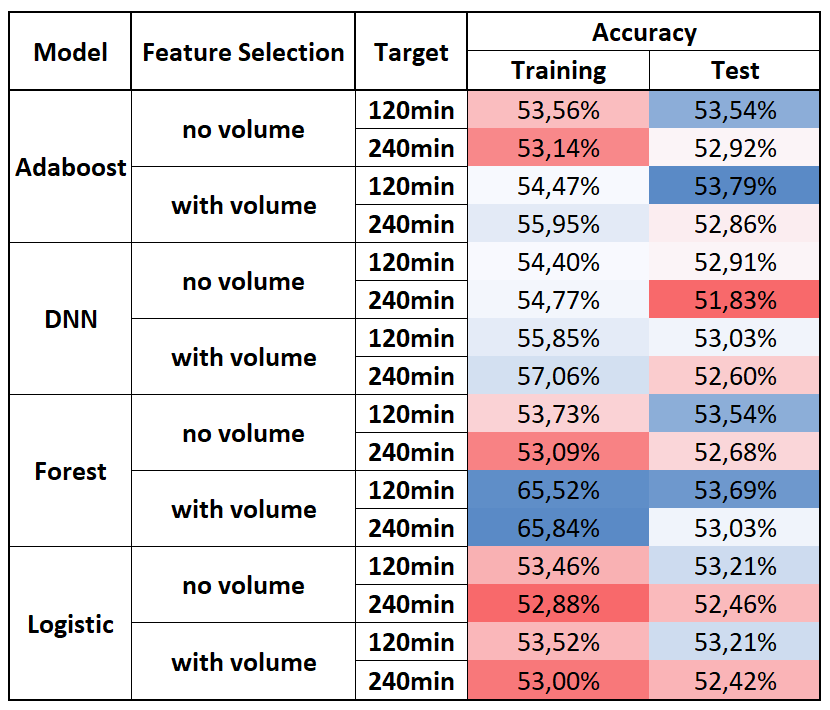
\includegraphics[width=165mm]{all/all_accuracy_train_test.png} }
    \caption{ 
        This table illustrates the accuracies for the different models being used on training
        and test set for different combinations of features and targets. 
        Red colors indicate relatively low and blue ones relatively high accuracies compared to the other respective training and test results.
    }
    \label{fig:all_accuracy_train_test}
\end{figure}


As one can see above, the accuracies are generaly fairly low for both training and test set,
which is not out of the ordinary when comparing the model performances to the results of other methods (see \cite{mcnally2018predictBTC}).
This indicates that the data contains a high amount of noise and low explanatory power, 
which supports the efficient market hypothesis. Even when including volume, the test accuracy remains low.

For the training set, the inclusion of volume increases the training accuracy when comparing the respective counterpart without volume.
This ought to be expected, since there are more features to fit the data with.
Methods such as DNN and Random Forest, which tend to fit the noise more closely, 
receive the greatest increase in training accuracy.
However, these increases in training accuracies do not translate to increases in test accuracy, which remain almost unchanged.

Changing the duration of an active position, i.e., increasing the lead $d$ from 120 to 240 min for target $ Y^{c}_{t + d, t} $ decreases test accuracies consistently.
This can be explained by the fact that price movements over longer periods of time exhibit greater variance,
thus leading to more uncertain predictions regarding price movements.
Since the accuracies for each model and specification are rather low in figure \ref{fig:all_accuracy_train_test}, 
one should consider increasing the threshold. Otherwise the correct trading decision signal get canceled out almost completely by the wrong ones.
Further, after introducing transaction costs for each trade, false trades can cause the overall return to drop considerably if conducted too often
which can be seen in chapter \ref{ch:strategy_performance}.


\begin{figure}[H]
    \captionsetup{format=plain}
    \makebox[\textwidth]{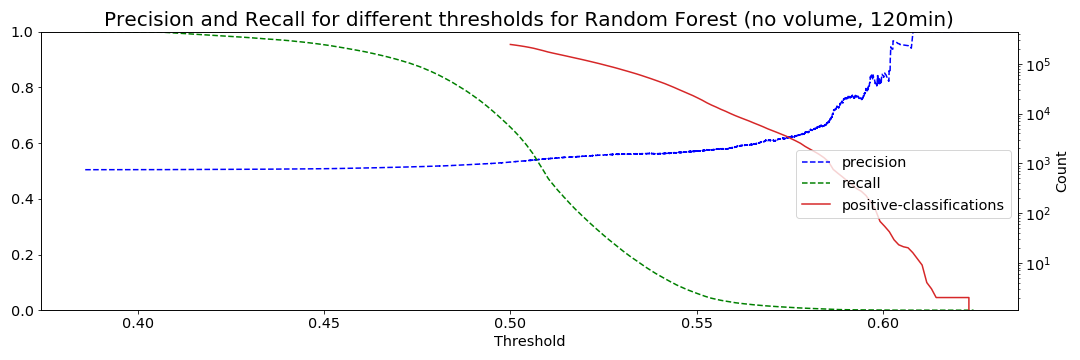
\includegraphics[width=165mm]{forest/rf_no_volume_future_2state_movement_120min_precision_vs_threshold.png} }
    \caption{ 
            This figure illustrates the precision, recall and up-classifications of the Random Forest for different thresholds
            without taking volume into consideration. 
        }
    \label{fig:rf_no_volume_future_2state_movement_120min_precision_vs_threshold}
\end{figure}


Figure \ref{fig:rf_no_volume_future_2state_movement_120min_precision_vs_threshold}
illustrates the tradeoff between precision and positive-classification for increasing tresholds.
When conducting trading with transaction cost, one should aim for increasing the precision, since false-positive decrease returns considerably.
However, by increasing the threshold in order to improve the precision, less positive-classifications, i.e., long position are conducted.
Thus, it is imperative to find a balance between precision and number of classifications.
In chapter \ref{ch:strategy_performance}, we demonstrate how changing thresholds leads to drastic
differences in terms of overall return.




\subsection{Strategy Performance} \label{ch:strategy_performance}

In this chapter, we outline the performance after employing the trading algorithm on the 
trading set as described in chapter \ref{ch:trading_algorithm}.
Figure \ref{fig:all_max_returns_15bps} below illustrates total maximum returns with 15bps transaction cost 
and its respective probability threshold for each model and specification.

\begin{figure}[H]
    \captionsetup{format=plain}
    \makebox[\textwidth]{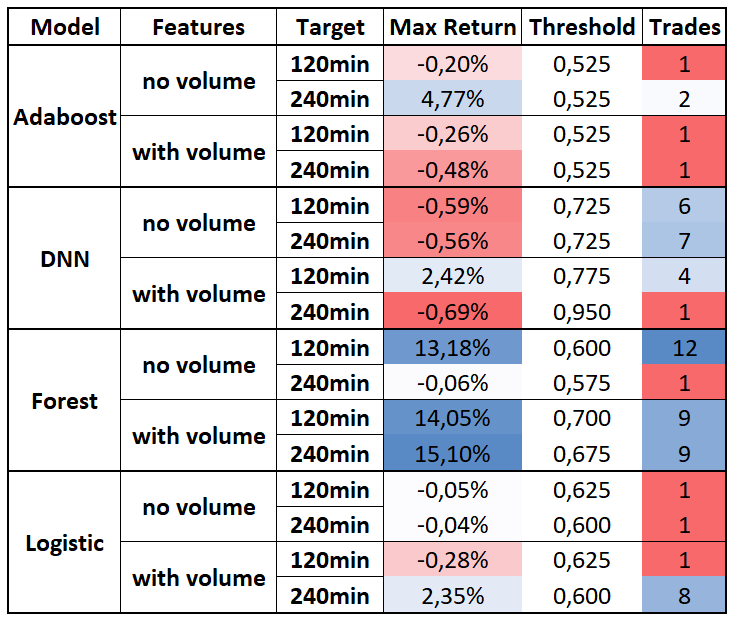
\includegraphics[width=165mm]{all/all_max_returns_15bps.png} }
    \caption{ 
            This figure illustrates the precision, recall and up-classifications of the Random Forest for different thresholds
            without taking volume into consideration. 
        }
    \label{fig:all_max_returns_15bps}
\end{figure}

Except for the random forest, which outperforms any other method significantly, most methods struggle to achieve positive returns.
AdaBoost, DNN, and Logistic Regression only generate negative returns, except for one feature and target specification combination.
Interestingly, this combination is different for each model, indicating no consistant explanatory power across models.
Compared to the 42\% short return of the equal-weight portfolio consisting of an equal investment in all ten coins and holding throughout
the trading period, the models are not able to beat simple holding diversified holding strategies.

Increasing the forecast duration from 120 to 240 min does not impact returns consistently with a correlation to returns of roughly -0,08. 
This indicates that the potential upside of higher price changes and less frequent transaction costs are mitigated 
by the increased difficulty for the model to predict the price movement. 
Also including volume has no consistent impact on returns.

The thresholds which maximize returns remain stable for AdaBoost and Logistic Regression across different specifications.
This is not the case for Random Forest and DNN for which this threshold is higher, which is indicative of a closer fit.
Further, the probability mass for the AdaBoost seems to be close to 0.5, 
since for a threshold of only 0,525 the number of conducted trades is between 1 and 2. This finding is also in line with the literature 
which states that decision trees and boosting methods, produce distorted class probability distributions
(see \cite{caruana2005probabilityDistortion} and \cite{zadrozny2005calibratedProbabilties}).
Figure \ref{fig:adaboost_no_volume_future_2state_movement_120min_precision_vs_threshold} illustrates precision, recall and up-classifications of the AdaBoost for different thresholds
without taking volume into consideration. One can see that, only slight increases in thresholds 
lead to drastic changes in precision and positive classifications. The Random Forest in figure \ref{fig:rf_no_volume_future_2state_movement_120min_precision_vs_threshold}
on the other hand exhibits a rather small changes for increasing thresholds.

\begin{figure}[H]
    \captionsetup{format=plain}
    \makebox[\textwidth]{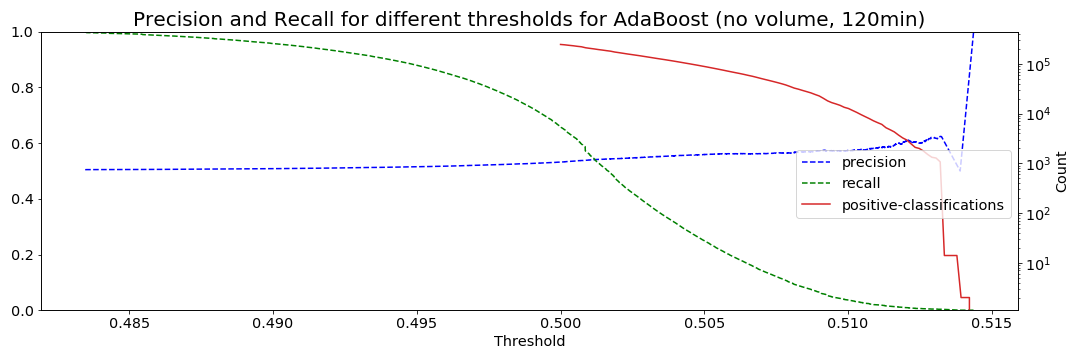
\includegraphics[width=165mm]{adaboost/adaboost_no_volume_future_2state_movement_120min_precision_vs_threshold.png} }
    \caption{ 
            This figure illustrates precision, recall and up-classifications of the AdaBoost for different thresholds
            with a prediction duration of 120min and only return features.
        }
    \label{fig:adaboost_no_volume_future_2state_movement_120min_precision_vs_threshold}
\end{figure}

On the hand, DNN and Random Forest do not have these biases
and predict less distorted probabilities, which is also supported by the literature \cite{caruana2005probabilityDistortion}. 
Overall, when calibrating the threshold to maximize returns, only a small amounts of trades are conducted for each model and specification.
This can be attributed to the aforementioned tradeoff between precision and positive-classifications when increasing the threshold, 
which is consistent across all specifications
(see appendix figure \ref{fig:adaboost_threshold_vs_precision} to \ref{fig:logistic_threshold_vs_precision}). 
However, only considering maximum returns, an interesting relationship emerges. 
The greater the number of trades conducted, the greater the maximum returns (correlation ~ 0,77), due to a higher amounts of profitable trades.
This is insofar surprising as a higher amount of trades due to lower thresholds consistently leads to less return as can be seen in figure 
\ref{fig:all_threshold_vs_return_15bps_no_volume_120min} below.

\begin{figure}[H]
    \captionsetup{format=plain}
    \makebox[\textwidth]{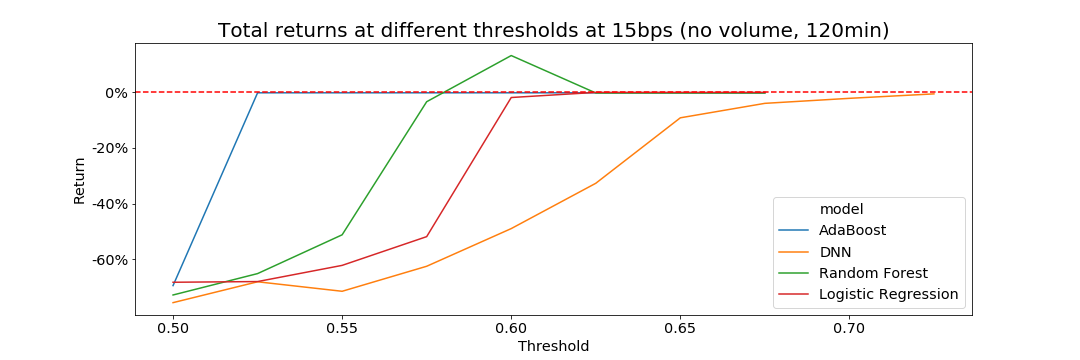
\includegraphics[width=200mm]{all/all_threshold_vs_return_15bps_no_volume_120min.png} }
    \caption{ 
            This figure illustrates total returns at a transaction cost of 15bps over the trading period for different thresholds.
            The four models were trained on features only containing returns and a forecast duration of 120min.
        }
    \label{fig:all_threshold_vs_return_15bps_no_volume_120min}
\end{figure}

All models start off with similar negative returns and converge to zero as the threshold progresses. 
This can be explained by the tradeoff illustrated in figure 
\ref{fig:adaboost_no_volume_future_2state_movement_120min_precision_vs_threshold} and \ref{fig:rf_no_volume_future_2state_movement_120min_precision_vs_threshold}
as the precision and accuracy is very low at thresholds near 0,5. 
The convergence is due to the small amount of trades occuring at higher thresholds, thus no trades are being conducted eventually.
This finding is consistent across models and specifications (see appendix figure \ref{fig:all_threshold_vs_return}).




\subsection{Further Analyses}
In this chapter, we analyse how the different return deltas impacted the predictions ofthe model.

Figure \ref{fig:forest_return_feature_importance_no_volume_120min} illustrates the feature importances for the Random Forest according to MDI \cite{louppe2015variableImportance}
for different return deltas in minutes (see chapter \ref{ch:feature_and_target}). 
For this particular graph, the Random Forest was trained on features containing only returns and a forecast duration of 120min.   
The overall shape resembles a concave graph peaking at around 80 min and then decreasing in importance.

\begin{figure}[H]
    \captionsetup{format=plain}
    \makebox[\textwidth]{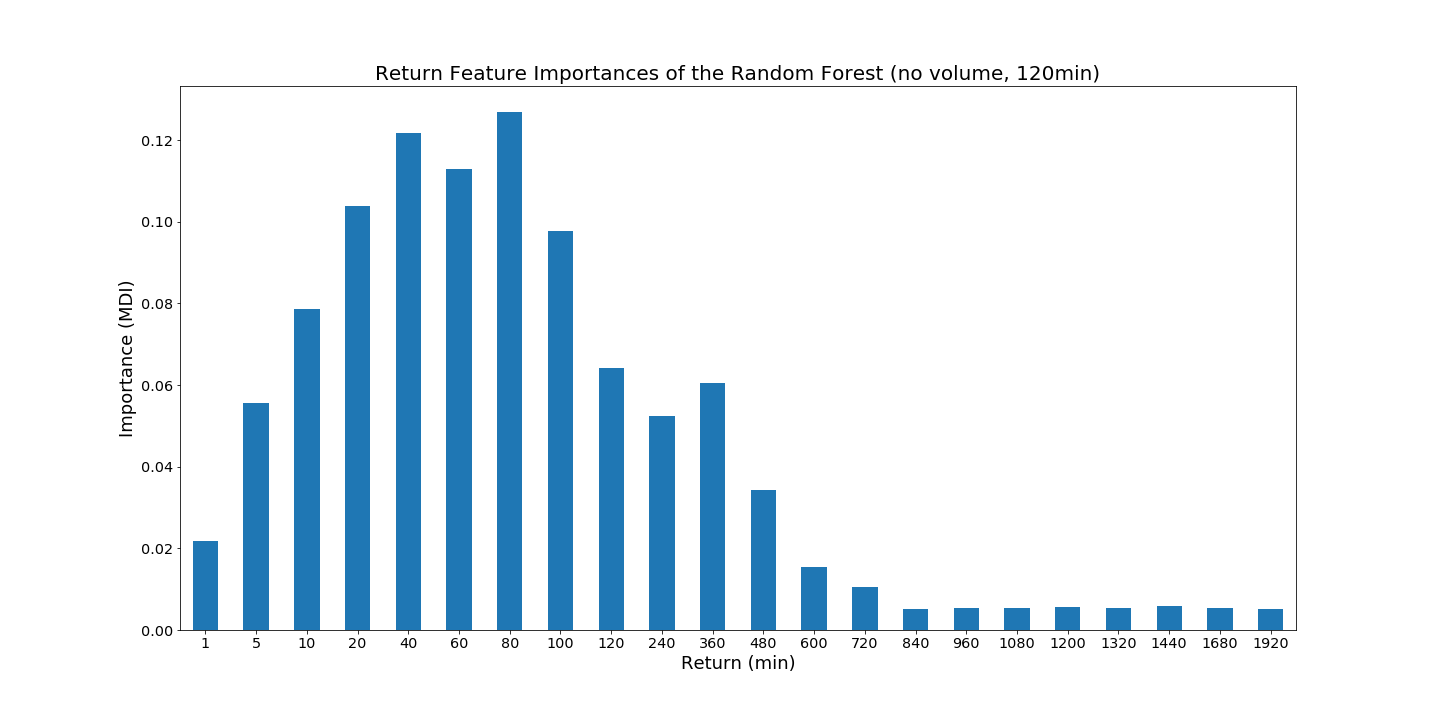
\includegraphics[width=200mm]{forest/forest_return_feature_importance_no_volume_future_2state_movement_120min.png} }
    \caption{ 
            This figure illustrates the feature importances of the Random Forest according to MDI \cite{louppe2015variableImportance}
            for different return deltas in minutes as described in chapter \ref{ch:training_trading}. 
            The Random Forest was trained on features containing only returns and a forecast duration of 120min.   
        }
    \label{fig:forest_return_feature_importance_no_volume_120min}
\end{figure}

As one can see, after a return delta of 10 hours, the relative importance remains low. 
This indicates that returns over a long period of time exhibit a relatively low explanatory power for
predicting price movements, while those near the middle of the forecast duration have the highest explanatory power.

\begin{figure}[H]
    \captionsetup{format=plain}
    \makebox[\textwidth]{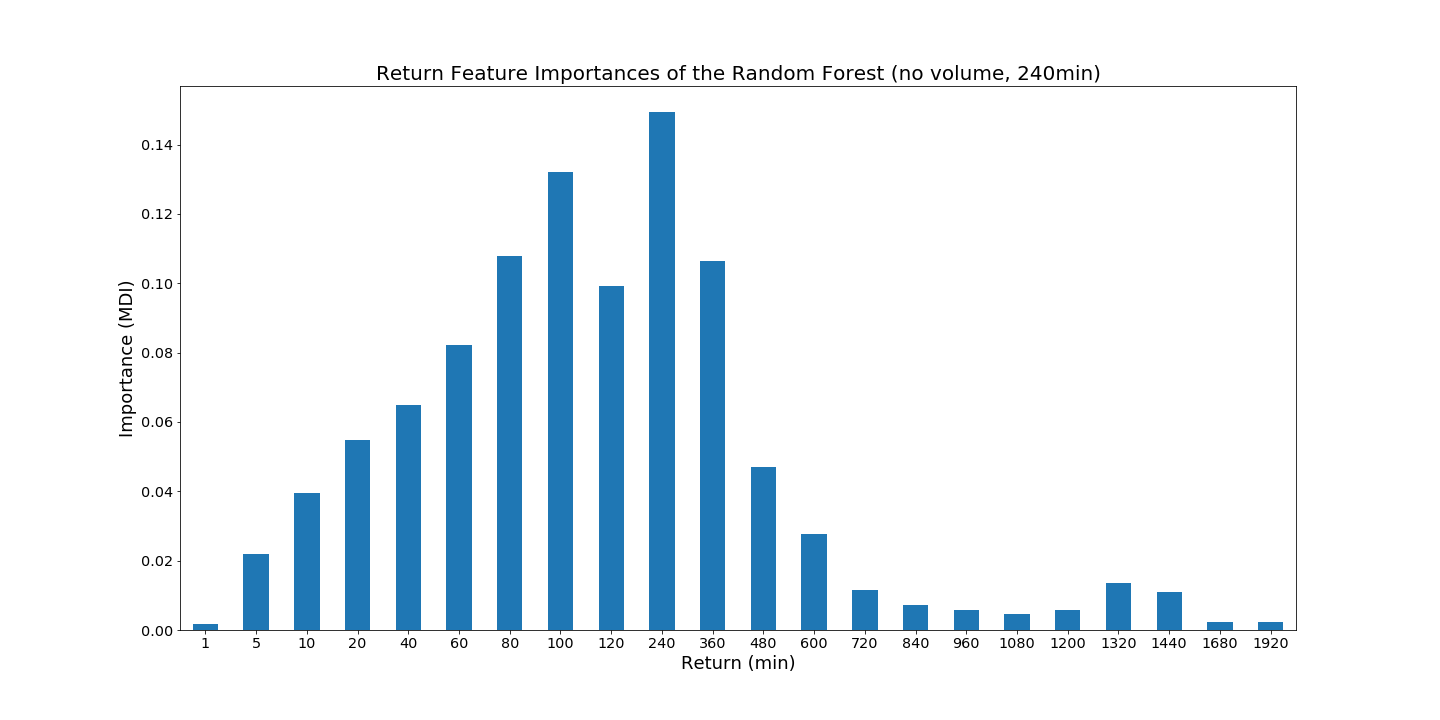
\includegraphics[width=200mm]{forest/forest_return_feature_importance_no_volume_future_2state_movement_240min.png} }
    \caption{ 
            This figure illustrates the feature importances of the Random Forest according to MDI \cite{louppe2015variableImportance}
            for different return deltas in minutes as described in chapter \ref{ch:training_trading}. 
            The Random Forest was trained on features containing only returns and a forecast duration of 240min.
        }
    \label{fig:forest_return_feature_importance_no_volume_240min}
\end{figure}

Extending the duration to 240min leads to similar feature importance pattern as can be seen in figure \ref{fig:forest_return_feature_importance_no_volume_240min}.
However, including volume in the feature selection leads to a radically different shape of feature importances 
as can be seen below in figure \ref{fig:forest_return_feature_importance_with_volume_120min}.

\begin{figure}[H]
    \captionsetup{format=plain}
    \makebox[\textwidth]{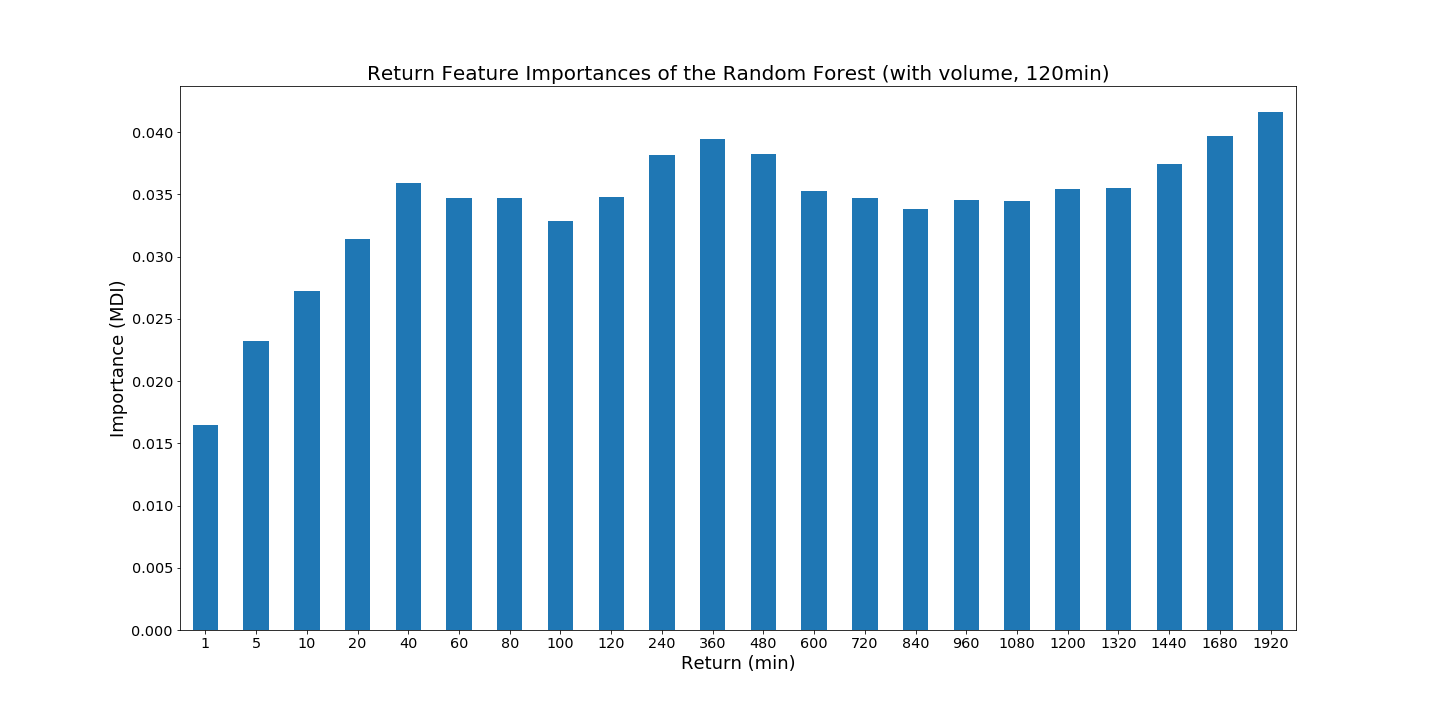
\includegraphics[width=200mm]{forest/forest_return_feature_importance_with_volume_future_2state_movement_120min.png} }
    \caption{ 
            This figure illustrates the feature importances of the Random Forest according to MDI \cite{louppe2015variableImportance}
            for different return deltas in minutes as described in chapter \ref{ch:training_trading}. 
            The Random Forest was trained on features containing both returns and volumes and a forecast duration of 120min.
        }
    \label{fig:forest_return_feature_importance_with_volume_120min}
\end{figure}

In addition, also the MDI values are consider lower than those in the graph without using volumes for the model fit. 
This indicates that the inclusion of volumes changes the relationship of returns and time for the Random Forest.
This is consistent across different forecast durations (see appendix figure \ref{fig:forest_return_feature_importance_with_volume_240min}).


Figure \ref{fig:logistic_return_coefficients_no_volume_120min} illustrates the coefficients of the Logistic Regression 
for different return deltas in minutes. Comparing the absolute coefficient values of with the MDI values 
from the Random Forest \cite{louppe2015variableImportance}, the relationship past return on forecasted future returns seems to be inverted. 
The highest coefficient values are realized at the beginning and near the end which is
in stark contrast to the Random Forest. Also this finding is consistent across specifications (see appendix figure \ref{fig:logistic_return_coefficients}), 
which was not the case for the Random Forest.
Due to the high interpretability of the Logistic Regression, 
one can also conclude that high returns in the first 600 min lead to low probability of an up-classification.
Thus, one can cautiously conclude that the Logistic Regression puts an emphasis on price stability, 
because is supposes a revertion of trend (down-movement after a series of positive returns and up-movement after a series of negative returns).



\begin{figure}[H]
    \captionsetup{format=plain}
    \makebox[\textwidth]{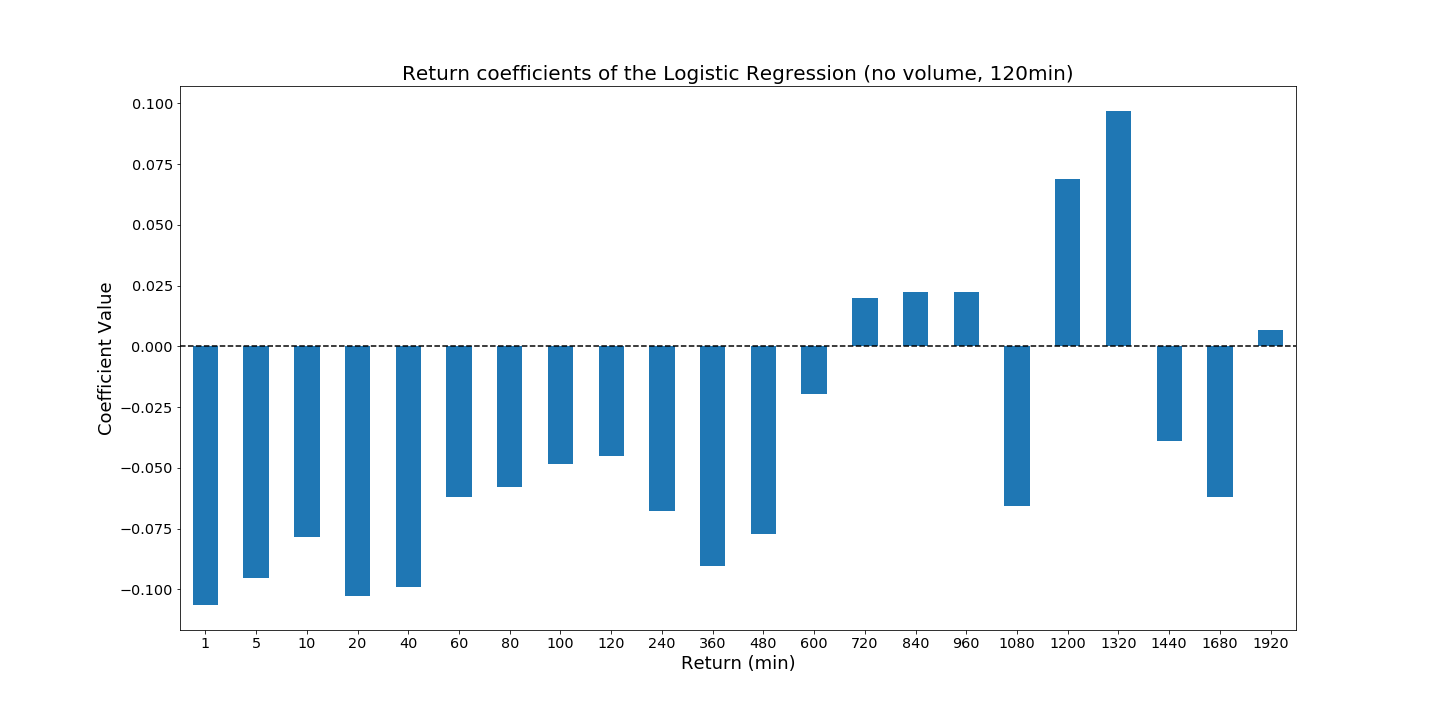
\includegraphics[width=200mm]{logistic/logistic_return_coefficients_no_volume_future_2state_movement_120min.png} }
    \caption{ 
            This figure illustrates the coefficients for the Logistic Regression 
            for different return deltas in minutes as described in chapter \ref{ch:training_trading}.
            The Logistic Regression was trained on features containing only returns and a forecast duration of 120min.
        }
    \label{fig:logistic_return_coefficients_no_volume_120min}
\end{figure}
